%! TEX root = teknologi_dalam_lingkungan.tex
% the main TeX file which is intended to compile, :VimtexReload after adjustment
   % this file should be included in the main file
% :h vimtex-tex-root
\documentclass[../wastek.tex]{subfiles}
%ensure the class of docs

\begin{document}

\section{Teknologi Ramah Lingkungan}%
\label{sec:teknologi_ramah_lingkungan}

\subsection{Pengertian dan Prinsip Teknologi Ramah Lingkungan}%
\label{sub:pengertian_dan_prinsip_teknologi_ramah_lingkungan}

Teknologi ramah lingkungan atau sering disebut dengan sustainable technology/green technology merupakan bentuk penerapan teknologi yang memperhatikan prinsip-prinsip pelestarian lingkungan. Teknologi tersebut bertujuan untuk memberi kemudahan dan pemenuhan keperluan manusia. Suatu teknologi dikatakan teknologi ramah lingkungan jika memenuhi syarat-syarat tertentu.

Teknologi ramah lingkungan bertujuan untuk menghasilkan berbagai produk dan jasa untuk kepentingan manusia. Teknologi tersebut memanfaatkan sumber daya alam yang dapat diperbarui dan tidak menghasilkan limbah yang membahayakan lingkungan. Selain itu, teknologi ramah lingkungan juga dapat menggunakan bahan yang dapat didaur ulang. Sumber energi listik dapat berasal dari matahari, angin, dan air. Sumber energi alternatif juga dipilih karena dapat diperbarui dan tidak mencemari lingkungan. Lingkungan sekitar kita tidak lepas dari pemanfaatan teknologi, mulai dari bidang pertanian, industri besar, dan industri skala rumah tangga. Pemanfaatan teknologi yang tidak tepat dapat mengakibatkan kerusakan pada lingkungan

\subsection{Aplikasi Teknologi Ramah Lingkungan}%
\label{sub:aplikasi_teknologi_ramah_lingkungan}

Teknologi ramah lingkungan telah diterapkan dalam berbagai bidang antara lain di bidang lingkungan.

\subsubsection{Biopori}%
\label{ssub:biopori}

Biopori dikenal dengan istilah teknologi lubang resapan (TLR), merupakan teknik untuk membuat wilayah resapan air hujan. Teknik biopori memiliki prinsip yang sama dengan sumur resapan. Teknik ini diterapkan dengan menyediakan area yang dibuat berlubang- lubang kecil (berpori) yang nantinya akan menyerap air hujan dan kemudian disalurkan ke dalam tempat penampungan air. Biopori sangat bermanfaat bagi pelestarian keseimbangan lingkungan.

\begin{figure}
	\begin{center}
		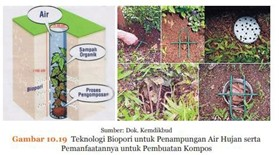
\includegraphics[width=.82\textwidth]{../figures/biopori.jpg}
		% filename may not contain space but _
	\end{center}
	\caption{Teknologi Biopori untuk Penampungan Air Hujan}
	\label{fig:}
\end{figure}


Selain dapat mencegah banjir pada musim hujan, biopori juga dapat menjamin ketersediaan air pada musim kemarau. Biopori juga dapat diandalkan untuk mencegah penyebaran penyakit yang disebabkan oleh adanya genangan air, seperti demam berdarah, malaria, dan kaki gajah. Kesuburan dan kelestarian organisme tanah juga dapat terjaga dengan teknologi ini. Lubang-lubang resapan air ini sekaligus juga dapat dimanfaatkan untuk membuat kompos, yakni dengan memberikan sampah organik seperti dedaunan atau sisa makanan.

\subsubsection{Fitoremediasi}%
\label{ssub:fitoremediasi}

Fitoremediasi merupakan salah satu bentuk bioremediasi. Fitoremediasi merupakan penggunaan tumbuhan untuk menghilangkan, memindahkan, menstabilkan, atau menghancurkan bahan pencemar baik itu senyawa organik maupun anorganik. Melalui fitoremediasi ini polutan (zat penyebab polusi) seperti logam berat, pestisida, minyak, dan zatlain yang mengotori tanah, air, atau udara dapat dikurangi bahkan dihilangkan. Fitoremediasi baru berkembang pada awal tahun 1990, yaitu dimulai dari kesuksesan dalam memperbaiki daerah tercemar oleh zat radioaktif sesium (Cs), stronsium (Sr), dan uranium (U) di Chernobyl, Rusia dengan menggunakan tumbuhan bunga matahari.
Keunggulan teknologi fitoremediasi ini antara lain: ramah lingkungan, biaya operasional rendah, mudah untuk diaplikasikan, aman digunakan, tanah dapat menjadi lebih subur, dan dapat membuat kualitas lingkungan menjadi lebih baik. Contoh tumbuhan yang dapat digunakan dalam fitoremediasi adalah bunga matahari (Helianthus annus), sawi (Brassica rappa), eceng gondok (Eichornia crassapies), padi (Oryza sativa), tembakau (Nicotiana tobacco), dan sansevieria (Sansevieria trifasciata).

\begin{figure}
	\begin{center}
		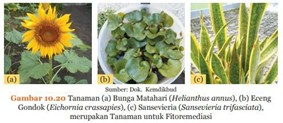
\includegraphics[width=.82\textwidth]{../figures/fitoremedi.jpg}
		% filename may not contain space but _
	\end{center}
	\caption{Tanaman untuk Fitoremediasi}
	\label{fig:tanaman_fitoremediasi}
\end{figure}

\subsubsection{Toilet Pengompos (Composting Toilet)}%
\label{ssub:toilet_pengompos_(composting_toilet)}
Composting toilet merupakan toilet kering yang menggunakan proses secara aerob untuk menghancurkan atau mendekomposisi feses yang dihasilkan manusia. Toilet pengompos dapat digunakan sebagai pengganti toilet air pada umumnya. Toilet ini biasanya ditambah dengan campuran serbuk gergaji, sabut kelapa, atau lumut tertentu untuk membantu proses aerob, menyerap air, dan mengurangi bau. Proses dekomposisi ini umumnya lebih cepat dari proses dekomposisi secara anaerob yang digunakan pada septic tank.

\subsubsection{Pemurnian Air (Water Purification)}%
\label{ssub:pemurnian_air_(water_purification)}

Percobaan mengenai pemurnian air pertama kali dilakukan pada abad ke-17. Sir Francis Bacon mencoba untuk mengambil garam dari air laut melalui saringan pasir. Meskipun percobaan ini belum berhasil, percobaan ini dikenal sebagai awal dari proses pemurnian air. Pemurnian air merupakan suatu proses penghilangan zat-zat kimia, kontaminan biologis, partikel-partikel padat, dan gas-gas dari air yang terkontaminasi atau kotor. Tujuan dari proses ini adalah untuk menghasilkan air yang dapat digunakan untuk keperluan tertentu. Secara umum, proses pemurnian air merupakan proses kajian fisika, kimia, dan biologi. Secara fisika, pada proses pemurnian air ada proses filtrasi atau penyaringan, sedimentasi atau pengendapan, dan distilasi atau penyulingan. Secara kimia, ada pemberian klorin (Cl2 ), penyinaran dengan sinar ultraviolet (UV), dan pemberian karbon aktif. Karbon aktif, klorin, dan sinar ultraviolet dapat berperan sebagai pembunuh kuman yang ada dalam air.

\begin{enumerate}

	\item Pemurnian Air Sederhana
	\item[] Pemurnian air dapat dilakukan dengan membuat alat yang berbentuk tabung yang di dalamnya terdapat lapisan-lapisan bahan seperti pasir, kerikil, batu, arang, ijuk atau sabut kelapa, dan dapat juga ditambah dengan kapas atau kain katun. Pada penjernihan air dilakukan proses penyaringan kotoran padat yang larut dalam air dengan pasir, kerikil, dan ijuk atau sabut kelapa. Air yang tersaring kotorannya akan melewati arang yang dapat mengurangi kumankuman dalam air. Air kotor dapat dituangkan ke dalam tabung melalui bagian atas tabung, selanjutnya air mengalir pada bagian bawah tabung karena adanya gaya gravitasi atau dibantu dengan tekanan dari luar. Selama mengalir ke bagian bawah tabung, air akan mengalami proses penyaringan sehingga pada bagian bawah dapat diperoleh air bersih.

	\item Teknologi Osmosis Balik

	\item[] Osmosis balik merupakan teknologi pemurnian air yang menggunakan prinsip kebalikan dengan prinsip osmosis. Osmosis balik menggunakan prinsip tekanan untuk mengatasi tekanan osmotik yang terjadi secara alami.
	      \begin{figure}
		      \begin{center}
			      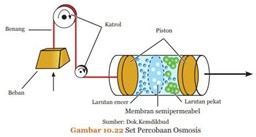
\includegraphics[width=.82\textwidth]{../figures/osmosis.jpg}
			      % filename may not contain space but _
		      \end{center}
		      \caption{Set percobaan Osmosis}
		      \label{fig:percobaan_osmosis}
	      \end{figure}

	\item[] Pada Gambar terdapat sebuah tabung yang berisi larutan garam dan diberi sebuah pemisah membran semipermeabel. Membran semipermeabel adalah suatu membran yang hanya dapat dilewati oleh molekul tertentu, tetapi tidak dapat dilalui oleh zat lainnya. Contoh zat yang dapat melalui membran semipermeabel adalah air. Pada proses osmosis, pelarut (misalnya air) secara alami berpindah dari daerah yang memiliki konsentrasi zat terlarut (misalnya garam) rendah (encer) melalui suatu membran menuju daerah yang memiliki konsentrasi zat terlarut tinggi (pekat). Pergerakan alami pelarut ini bertujuan untuk menyamakan konsentrasi zat terlarut pada kedua sisi bagian membran.
	\item[] Perhatikan mekanisme osmosis balik pada gambar berikut. Pada osmosis balik, pelarut seperti air akan bergerak dari larutan yang pekat ke larutan yang encer. Hal tersebut dapat terjadi karena adanya tekanan dari luar sehingga dapat membalik arah aliran secara alami. Adanya tekanan dari luar akan menyebabkan air dari larutan yang pekat mengalir ke arah larutan encer, sehingga dapat dihasilkan air yang tidak mengandung garam. Teknologi osmosis balik ini diterapkan dalam pembuatan air minum dari air laut, yakni dengan menghilangkan garam dan zat-zat lain yang tercampur dengan molekul air.

\end{enumerate}
\begin{figure}
	\begin{center}
		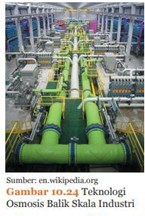
\includegraphics[width=.82\textwidth]{../figures/osmosis_industri.jpg}
		% filename may not contain space but _
	\end{center}
	\caption{Teknologi osmosis Balik Skala Industri}
	\label{fig:osmosis_industri}
\end{figure}

\subsection{Teknologi Pengolahan Sampah}%
\label{sub:teknologi_pengolahan_sampah}

Terdapat beberapa teknologi pengolahan yang dapat diterapkan. Berdasarkan SNI 19-2454-2002 tentang Tata cara teknik operasional pengelolaan sampah perkotaan, teknik pengolahan sampah, terdapat beberapa teknik pengolahan sampah, antara lain:
\begin{itemize}
	\item Pengomposan
	      \begin{itemize}
		      \item Berdasarkan kapasitas (individual, komunal, skala lingkungan)
		      \item Berdasarkan proses (alami, biologis dengan cacing, biologis dengan mikro organisme tambahan)
	      \end{itemize}
	\item Insinerasi yang berwawasan lingkungan
	\item Daur ulang
	      \begin{itemize}
		      \item Sampah an organic disesuaikan dengan jenis sampah
		      \item Menggunakan kembali sampah organic sebagai makanan ternak
	      \end{itemize}
	\item Pengurangan volume sampah dengan pencacahan atau pemadatan
	\item Biogasifikasi (pemanfataan energi hasil pengolahan sampah)
\end{itemize}

\begin{table}[htb]
	\caption{Kelebihan dan kelemahan alternatif sistem pengelolaan sampah}
	\label{tb:nome}
	\begin{tabularx}{\textwidth}{p{3cm} X X X}
		\hline
		Jenis Pengolahan                               &  Kelebihan  &  Kelemahan  &  Catatan  \\
		\hline

		Composting (High rate/modern)                  &
		\tabitem Proses pengomposan lebih cepat
		\tabitem Volume sampah berkurang               &
		\tabitem Memerlukan peralatan kompleks
		\tabitem Biaya investasi mahal                 &
		Harga kompos lebih mahal dari pupuk kimia; biaya operasi tinggi  \\[0.5em]

		Windrow composting (sederhana)                 &
		\tabitem Tidak memerlukan banyak peralatan
		\tabitem Cocok untuk sampah organik
		\tabitem Volume sampah berkurang
		\tabitem Biaya investasi murah                 &
		\tabitem Perlu perawatan kontinu
		\tabitem Proses lebih lama
		\tabitem Membutuhkan tenaga lebih banyak       &
		-  \\[0.5em]

		Pemadatan                                      &
		\tabitem Volume sampah berkurang
		\tabitem Efisien untuk pengangkutan            &
		Biaya investasi dan operasional relatif mahal  &
		Dianjurkan jika jarak ke TPA > 25 km  \\[0.5em]

		Insinerasi (Pembakaran)                        &
		\tabitem Cocok untuk kapasitas besar
		\tabitem Dapat menghasilkan energi listrik
		\tabitem Volume sangat berkurang
		\tabitem Higienis                              &
		\tabitem Biaya investasi dan operasi mahal
		\tabitem Berpotensi polusi udara               &
		Ada 2 tipe: kontinu (>100 ton/hari) dan terputus (<100 ton/hari)  \\[0.5em]

		Recycling (Daur ulang)                         &
		\tabitem Pemanfaatan kembali bahan anorganik
		\tabitem Membuka lapangan kerja informal
		\tabitem Mengurangi volume sampah              &
		\tabitem Tidak semua sampah bisa didaur ulang
		\tabitem Peralatan mekanis mahal
		\tabitem Kurang sehat bagi pekerja informal    &
		Dianjurkan pemisahan dari sumber sampah  \\

		\hline
	\end{tabularx}
\end{table}

\subsubsection{Teknologi Pemilahan}%
\label{ssub:teknologi_pemilahan}

Salah satu cara yang dapat digunakan untuk meminimalkan timbulan sampah di TPA adalah pemilahan sampah sejak di sumber. Pengumpulan sampah secara terpisah sudah mulai diterapkan di Negara German pada tahun 1893, yaitu dengan memisahkan wadah sampah kering, debu atau butiran, dan sampah organik.
Seiring perkembangan jaman, proses pemilahan sampah tidak lagi dilakukan secara manual, tetapi menggunakan mesin atau dilakukan secara mekanik.
Pada perkembangannya, pemilahan sampah secara mekanis dilakukan secara terintegrasi dalam suatu unit pemilahan mekanis. Tidak jarang, pengolahan secara mekanis tersebut berlanjut dengan pengolahan biologis. Integrasi pengolahan mekanis dan biologis ini dikenal dengan teknologi Mechanical Biological Treatment (MBT).

Mechanical Biological Treatment (MBT).
MBT merupakan integrasi dari proses pengolahan biologis dan mekanis. Berikut disajikan skema pengolahan mekanis, skema pengolahan biologis dan integrasi dari kedua pengolahan tersebut.


Prinsip kerja dari MBT adalah pemilahan material dengan beberapa tujuan, yaitu:
\begin{itemize}
	\item Memisahkan material untuk recovery energi
	\item Memisahkan material untuk recovery material
	\item Memisahkan material untuk mempermudah proses pengolahan biologis
\end{itemize}

Setelah mengalami pemisahan, material-material tersebut akan mengalami dua proses dasar pengolahan yaitu stabilisasi dan pengeringan sampah untuk recovery energi dan pengolahan sampah untuk mengurangi emisi yang akan ditimbulkan landfill. MBT menerapkan system pengolahan yang berbeda untuk setiap tipe material sampah. Sampah dengan kandungan air yang tinggi akan mengalami proses pengolahan biologis dengan tahapan aerated windrow heap composting. Sedangkan pada tahap mekanik, tipe material ini akan melalui proses shredder, sieving drum, magnetic separator, dan sorting. Material dengan kandungan air yang rendah akan mengalami tahap mekanis terlebih dahulu sebelum menjalani proses pengolahan secara biologis. Proses mekanis yang dilalui berupa sieving drum, magnetic separator, sorting cabin. Sedangkan proses biologisnya tetap menggunakan aerated windrow heap composting.

\begin{figure}
	\begin{center}
		
\includegraphics[width=.82\textwidth]{tahap_pengelolaan_mbt}
		% filename may not contain space but _
	\end{center}
	\caption{Tahap pengolahan mekanis dalam MBT}
	\label{fig:tahap_mbp}
\end{figure}


\subsubsection{Anaerobik Digester}%
\label{ssub:anaerobik_digester}

Proses anaerob adalah proses pengolahan secara biologi yang terjadi tanpa kehadiran oksigen. Pengolahan secara anaerob dilakukan oleh mikroorganisme fakultatif dan obligat anaerob, dimana tanpa kehadiran oksigen akan mengubah senyawa organic menjadi gas sebagai hasil akhir semacam karbondioksida dan metana. Pada proses anaerob yang menjadi akseptor electron adalah senyawa organic dari perubahan organic menjadi CH4. Fermentasi anaerob membutuhkan organisme lain dalam mendegradasi senyawa organic menjadi metan karena terbatasnya jumlah substratyang dikatabolisme oleh bakteri metanogen (Sawatdeenarunat, 2006).

Anaerobic digestion (AD) serupa dengan pengomposan tetapi dalam kondisi tanpa oksigen. Terdapat berbagai variasi anaerobic digestion yang meliputi (Juniper, 2005):
\begin{itemize}
	\item Proses kering (penambahan air minimal) dan basah (suspense atau slurry)
	\item Proses mesofilik (35o) dan termofilik (55oC)
	\item Proses satu tahap dan dua tahap
	\item Perkolasi, hidrolisis dan fermentasi dari fasa yang mengandung air
	\item Proses interval (aerobic-anaerobik-aerobik)
\end{itemize}

Digestion dibagi menjadi dua kelompok berdasarkan kandungan airnya, yaitu fermentasi kering dengan kadar padatan terlarut > 25\% dan fermentasi basah dengan kadar padatan terlarut <15\%. Anaerobi digestion pada umumnya dikombinasikan dengan tahap dari proses pengomposan karena tidak semua substansi organic dapat didegradasi dalam kondisi anaerob.

Anaerobic digestion wet (basah) membutuhkan biaya operasional yang lebih tinggi dibanding dengan anaerobic digestion dry (kering). Pada system basah, proses degradasi menghasilkan lebih banyak residu berupa air sehingga operasional anaerobic digestion juga harus dilengkapi dengan sarana pengolahan efluen tersebut. Keuntungan dari system kering adalah permasalahan seperti settling, foaming, dan flotasi yang sering muncul pada system basah dapat dihindari. Namun anaerobic digestion kering sangat ditentukan oleh material input, sehingga proses ini sangat bergantung pada pengadukan eksternal dari input sampah untuk homogenitas.

\subsubsection{Composting (pengomposan)}%
\label{ssub:composting_(pengomposan)}
Kompos didefinisikan sejenis pupuk organik, dimana kandungan unsur N, P dan K yang tidak terlalu tinggi , hal ini membedakan kompos dengan pupuk buatan. Kompos sangat banyak mengandung unsur hara mikro yang berfungsi membantu memperbaiki struktur tanah dengan meningkatkan porositas tanah sehingga tanah menjadi gembur dan lebih mampu menyimpan air (Tchobanoglous et al.,1993). Adapun manfaat dari kompos adalah :

Memperbaiki struktur tanah;
\begin{itemize}
	\item Sebagai bahan baku pupuk organik;
	\item Sebagai media remediasi tanah yang tercemar (pemulih tanah akibapencemaran bahan kimia yang toxic terhadap mikroba tanah);
	\item Meningkatkan oksigen dalam tanah;
	\item Menjaga kesuburan tanah;
	\item Mengurangi kebutuhan pupuk inorganik.
\end{itemize}

Cara atau metoda untuk membuat kompos adalah proses komposting. Proses komposting ini merupakan proses dengan memanfaatkan proses biologis yaitu pengembangan massa mikroba yang dapat tumbuh selama proses terjadi. Metoda ini adalah proses biologi yang mendekomposisi sampah (terutama sampah organic yang basah) menjadi kompos karena adanya interaksi kompleks dari organisme yang terdapat secara alami. Berdasarkan prinsip proses biologis ini, maka karakteristik dari mikroba menjadi penting untuk diperhatikan. Jenis mikroba yang dimaksud adalah jenis mikroba yang diklasifikasikan dari cara hidupnya, yaitu :

\begin{itemize}
	\item Mikroba anarobik (yaitu mikroba yang hidup tanpa oksigen); jenis mikroba ini juga dibagi dalam 2 jenis, yaitu: mesofilik (hidup pada temperature 20-40oC), dan thermophilic (hidup pada temperature 45-70oC)
	\item Mikroba aerobic adalah mikroba yang hanya dapat hidup dengan adanya oksigen. Sama dengan mikroba anaerobic berdasarkan fluktuasi kondisi suhu di dalam tumpukan kompos dapat dibedakan menjadi mesophilic dan thermophilic.
\end{itemize}
Proses komposting merupakan suatu proses yang paling relatif mudah dan murah, serta menimbulkan dampak lingkungan yang paling rendah. Proses ini hampir sama dengan pembusukan secara lamiah, dimana berbagai jenis mikroorganisme berperan secara serentak dalam habitatnya masing-masing. Makanan untuk mikorooganisme adalah sampah, sedangkan suplai udara dan air diatur dalam proses komposting ini.

Jenis sampah sangat mempengaruhi proses composting ini. Sampah yang dapat dikomposkan adalah sampah organik atau sering disebut sampah basah adalah jenis sampah yang berasal dari jasad hidup sehingga mudah membusuk dan dapat hancur secara alami. Contohnya adalah sayuran, daging, ikan, nasi, ampas perasan kelapa, dan potongan rumput /daun/ ranting dari kebun.


\begin{figure}
	\begin{center}
		
\includegraphics[width=.82\textwidth]{sampah_kompos}
		% filename may not contain space but _
	\end{center}
	\caption{Sampah yang dapat dikomposkan}
	\label{fig:sampah_kompos}
\end{figure}

Berdasarkan teknologi proses, pengolahan kompos dapat dibedakan menjadi komposting \textbf{aerobik} dan \textbf{anaerobik}.

\subsubsection{Pirolisis dan Gasifikasi}%
\label{ssub:pirolisis_dan_gasifikasi}
\textbf{Pirolisis}

Pirolisis adalah degradasi limbah organic secara thermal dalam kondisi tanpa oksigen untuk menghasilkan arang karbon, minyak dan gas yang dapat dibakar. Besarnya produk yang akan dihasilkan dipengaruhi kondisi proses, terutama temperature dan laju pemanasan. Perbedaan utama antara pirolisis, gasifikasi, dan insinerasi terdapat pada jumlah oksigen yang disuplai ke reactor thermal. Pirolisis berjalan tanpa kehadiran oksigen dan gasifikasi menggunakan suplai oksigen yang terbatas. Melalui kedua proses tersebut pembakaran sempurna tidak terbentuk, sehingga selain gas yang dapat dibakar, karbon monoksida dan hydrogen juga akan dihasilkan. Oksigen untuk gasifikasi disuplai dalam bentuk udara, panas, atau oksigen murni. Insinerasi melibatkan oksidasi sempurna dari limbah dalam kondisi suplai oksigen berlebih untuk menghasilkan karbon dioksida, air dan abu, ditambah beberapa produk seperti logam, trace hidrokarbon, gas asam, dan lain-lain.

\textbf{Gasifikasi}
Gasifikasi adalah suatu teknologi proses yang mengubah bahan padat menjadi gas. Bahan padat yang dimaksud adalah bahan bakar padat, termasuk diantaranya biomassam batubara, dan arang. Gas yang dimaksud adalah gas-gas yang keluar dari proses gasifikasi dan umumnya berbentuk CO, CO2, H2, dan CH4. Proses gasifikasi dati limbah terjadi pada temperature yang lebih tinggi dari pirolisis dan dengan penambahan oksigen yang terkontrol. Produk berupa campuran hgas CO dan H2 dikenal sebagai syngas dan bisa digunakan sebagai substitusi gas alami. Reaksi dasar gasifikasi adalah sebagai berikut.

\[
	\mathrm{C}_n\mathrm{H}_m + 0{,}55n\,\mathrm{O}_2 \rightarrow n\,\mathrm{CO} + 0{,}5m\,\mathrm{H}_2
\]

Proses gasifikasi pada hakikatnya mengoksidasi suplai hidrokarbon pada lingkungan yang terkontrol untuk memproduksi gas sintetis yang memiliki nilai komersial yang signifikan. Gasifikasi adalah suatu alternative yang menarik karena proses ini mencegah pembentukan dioksin dan senyawa aromatic. Proses gasifikasi juga menghasilkan reduksi utama pada volume input limbah rata-rata sekitar 75\%.

Gasifikasi berbeda denagn pirolisis dan pembakaran. Ketiganya dibedakan berdasrkan kebutuhan udara yang diperlukan selama proses. Jika jumlah udara: bahan bakar (AFR, Air Fuel Ratio) sama dengan 0, maka proses disebut pirolisis. Jika AFR yang diperlukan selama proses kurang dari 1,5, maka proses disebut gasifikasi. Jika AFR yang diperlukan lebih dari 1,5, maka proses disebut proses pembakaran.

\subsubsection{Daur Ulang Sampah}%
\label{ssub:daur_ulang_sampah}

Daur ulang didefinisikan suatu proses mengumpulkan, memisahkan, melakukan proses, menjual material yang dapat dimanfaatkan kembali atau mengubah menjadi material baru. Dalam pengelolaan sampah terpadu daur ulang merupakan salah satu bagian penting yang ditunjukkan dengan hirarki sebagai berikut.

\begin{figure}
	\begin{center}
		
\includegraphics[width=.82\textwidth]{hirearki_olahan_sampah}
		% filename may not contain space but _
	\end{center}
	\caption{Hirarki pengelolaan sampah}
	\label{fig:hirearki_olahan_sampah}
\end{figure}

Daur ulang adalah salah satu komponen dalam hirarki pengelolaan sampah. Konsep daur-ulang (recycle) mengandung pengertian pemanfaatan semaksimal mungkin residu melalui proses, baik sebagai bahan baku untuk produk sejenis seperti asalnya, atau sebagai bahan baku untuk produk yang berbeda, atau memanfaatkan enersi yang dihasilkan dari proses recycling tersebut (Damanhuri \& Tri Padmi, 2010). Mengubah bentuk dan sifat sampah melalui proses bio-fisik- kimiawi menjadi produk baru (sampah basah diolah menjadi kompos, sampah plastik diolah menjadi pellet.


\subsubsection{Stasiun Peralihan Antara (SPA)}%
\label{ssub:stasiun_peralihan_antara_(spa)}

Didalam sistem penanganan sampah, SPA Skala Kawasan merupakan bagian dari kegiatan pengolahan antara dengan tujuan mereduksi volume sampah sebelum diangkut ke TPA dan atau TPST, dan atau pengguna akhir olahan sampah. Fungsi SPA antara lain sebagai tempat untuk proses reduksi volume, sebelum diangkut ke TPA dan atau TPST dan atau pengguna akhir olahan sampah. Selain itu SPA berfungsi untuk tempat pemindahan sampah dari kendaraan pengumpul kecil ke kendaraan pengangkut besar dan sebagai tempat pemindahan tanggung jawab penanganan sampah, dari pengumpul sampah ke penanggung jawab penanganan sampah.

Terdapat beberapa manfaat yan g dapat diambil dari penggunaan SPA, antara lain mengurangi jumlah dan atau volume sampah terangkut ke TPA melalui proses pemadatan, salah satu upaya mengurangi biaya pengangkutan sampah ke TPA dengan adanya reduksi kebutuhan ritasi kendaraan angkut ke TPS dan atau TPST, atau ke lokasi pemrosesan akhir lainnya, memperpanjang Umur TPA dengan pola pemrosesan penimbunan (landfiling), sebagai solusi bagi Pemerintah Kota dan atau Kabupaten dalam menangani permasalahan kesulitasn lahan TPA di dalam kota, dan tingginya beban pengangkutan.


\subsection{Teknologi Pengendalian Pencemaran Udara}%
\label{sub:teknologi_pengendalian_pencemaran_udara}

Teknologi pengendalian pencemaran udara dalam suatu plant atau tahap proses dirancang untuk memenuhi kebutuhan proses itu atau perlindungan lingkungan. Teknologi ini dapat dipilih dengan penerapan susunan alat pengendali sehingga memenuhi persyaratan yang telah disusun dalam rancangan proses.


Rancangan proses pengendalian pencemaran ini harus dapat memenuhi persyaratan yang dicantumkan dalam peraturan pengelolaan lingkungan. Rancangan ini harus mempertimbangkan factor ekonomi. Jadi penerapan peralatan pengendalian ini perlu dikaitkan dengan perkembangan proses produksi itu sendiri sehingga memberikan nilai ekonomik yang paling rendah baik untuk instalasi, operasi dan pemeliharaan. Nilai ekonomik yang dihubungkan dengan biaya produksi ini masih sering dianggap cukup besar. Penilaian ekonomik yang dihubungkan dengan kemaslahatan masyarakat kurang ditinjau, karena analisis ini kurang dapat dipahami oleh pihak industriawan. Dengan demikian penerapan peraturan harus dilaksanakan dan diawasi dengan baik, agar penerapan teknologi pengendalian ini bukan hanya sekedar memasang alat pengendalian pencemaran udaram tetapi kinerja alat ini tidak memenuhi persyaratan.


Teknologi pengendalian ini perlu dikaji dengan seksama, agar penggunaan alat tidak berlebihan dan kinerja yang diajukan oleh pembuat alat dapat dicapai dan memenuhi persyaratan perlindungan lingkungan. System pengendalian ini harus diawali dengan memahami watak emisi senyawa pencemar dan lingkungan penerima. Teknologi pengendalian yang sempurna akan membutuhkan biaya yang besar sekali sehubungan dengan dimensi alat, kebutuhan energy, keselamatan kerja dan mekanisme reaksi.


Faktor-faktor yang mempengaruhi dalam pemilihan teknologi pengendalian atau rancangan system pengendalian meliputi:
\begin{itemize}
	\item Watak gas buang atau efluen
	\item Tingkat pengurangan yang dibutuhkan
	\item Teknologi komponen alat pengendalian pencemaran
	\item Kemungkinan perolehan senyawapencemar yang bernilai ekonomik.
\end{itemize}
Watak efluen merupakan factor penentu dan tidak dapat digunakan untuk penyelesaian semua jenis pengendalian pencemaran. Jadi watak fisik kimia dan eluen dan lingkungan penerima harus di fahami dengan baik. Kemungkinan fenomena sinergetik yang dapat berlangsung harus dapat di perkirakan, jika perubahan watak atau komposisi effluent atau proses produksi dapat berlangsung dalam waktu yang akan dating.


Rancangan system penglolaan udara di daerah industry meliputi semua langkah perbaikan dan metode perlakuan yang menjamin hasil guna yang ekonomis untuk penyelesaian masalah.

\subsubsection{Gravitational Settler}%
\label{ssub:gravitational_settler}
Settling Chamber adalah alat pengendali partikulat pertama yang sering dipakai untuk menurunkan emisi debu. Saat ini sudah jarang dipakai karena tingkat efisiensinya yang rendah untuk patikel berukuran kecil.

Prinsip penyisihan partikulat dalam Gravity Settler, yaitu gas yang mengandung partikulat dialirkan melalui suatu ruang (chamber) dengan kecepatan rendah sehingga memberikan waktu yang cukup bagi partikulat untuk mengendap secara gravitasi ke bagian pengumpul debu (dust collecting hoppers).

Keuntungan

\begin{itemize}
	\item Kehilangan tekanan rendah
	\item Mudah dalam desain dan pemeliharaan
\end{itemize}
Kerugian :

\begin{itemize}
	\item Kebutuhan ruang besar
	\item Harus dibersihkan secara manual
	\item Efisiensi rendah yaitu kurang dari 50\%
\end{itemize}

\begin{figure}
	\begin{center}
		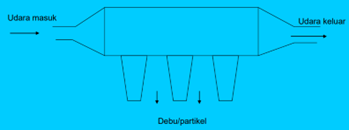
\includegraphics[width=.82\textwidth]{../figures/settler.png}
		% filename may not contain space but _
	\end{center}
	\caption{Gravitational Settler}
	\label{fig:settler}
\end{figure}

\subsubsection{Siklon}%
\label{ssub:siklon}

Siklon adalah suatu peralatan mekanis yang digunakan untuk menyisihkan partikel dengan ukuran relatif besar dari suatu aliran gas. Memiliki bentuk yang khas, dapat ditempatkan di atap dari suatu instalasi atau di samping bangunan. Siklon diguanakan sebagai precleaner, didesain untuk menyisihkan >80\% kandungan partikel yang berdiameter >20 mikron.

\begin{figure}
	\begin{center}
		
\includegraphics[width=.82\textwidth]{siklom}
		% filename may not contain space but _
	\end{center}
	\caption{Siklon}
	\label{fig:siklon}
\end{figure}


Prinsip penyisihan Siklon yaitu aliran gas bermuatan partikel memasuki siklon dan bergerak ke bawah akibat gaya sentrifugal dan gaya inersia dengan aliran berbentuk spiral, sedangkan partikel berukuran tertentu terlempar ke luar aliran spiral dan

berbenturan dengan dinding siklon, lalu terendapkan pada bagian dasar siklon. Di dekat dasar siklon, aliran gas berbalik arah bergerak ke atas dalam putaran spiral (vorteks) yang lebih kecil, dan keluar lewat outlet pada bagian atas siklon.


Keuntungan :

\begin{itemize}
	\item Mudah dalam desain dan pemeliharaan
	\item Kebutuhan luas ruang kecil
	\item Dapat dioperasikan pada temperatur tinggi
	\item Kehilangan tekanan rendah
\end{itemize}

Kerugian :
\begin{itemize}
	\item Butuh ruangan yang tinggi
	\item Rendah efisiensi untuk partikel kecil
	\item Sensitif pada debit udara dan beban yang bervariasi
	\item Biaya operasi tinggi
\end{itemize}

\subsubsection{Elektrostatic Precipitator}%
\label{ssub:elektrostatic_precipitator}

\begin{figure}
	\begin{center}
		
\includegraphics[width=.82\textwidth]{elektrostatic}
		% filename may not contain space but _
	\end{center}
	\caption{Elektrostatic Precipatator}
	\label{fig:elektrostatic}
\end{figure}


Electrostatic Precipitator (EP) adalah alat pengendali pencemar partikulat yang didasari pada konsep presipitasi akibat gaya elektrostatik. Sangat efektif sebagai pengendali partikulat yang berukuran <10 mikron.

Cara kerja dari electro static precipitator (ESP) adalah (1) melewatkan gas buang (flue gas) melalui suatu medan listrik yang terbentuk antara discharge electrode dengan collector plate, flue gas yang mengandung butiran debu pada awalnya bermuatan netral dan pada saat melewati medan listrik, partikel debu tersebut akan terionisasi sehingga partikel debu tersebut menjadi bermuatan negatif (-). (2) Partikel debu yang sekarang bermuatan negatif (-) kemudian menempel pada pelat-pelat pengumpul (collector plate).

Kelebihan :

\begin{itemize}
	\item Efisiensi penyisihan partikel sangat tinggi
	\item Mampu menyisihkan partikel berukuran kecil
	\item Dapat menangani debit aliran gas besar dengan kehilangan tekan yang rendah.
	\item Dapat digunakan untuk pengumpul sistem kering bagi materi yang bernilai, atau pengumpul sistem basah untuk fume dan mist
	\item Dapat didesain aliran gas dengan temperatur cukup tinggi
	\item Biaya operasi rendah, kecuali untuk efisiensi yang sangat tinggi.
\end{itemize}


Kekurangan :

\begin{itemize}
	\item Capital cost yang tinggi
	\item Hanya menyisihkan partikulat dan tidak dapat menyisihkan pencemar dalam bentuk gas
	\item Tidak terlalu fleksibel
	\item Memerlukan lahan yang luas
	\item Ozon dihasilkan dari pemberian muatan negatif terhadap elektroda pada saat ionisasi gas
	\item Dibutuhkan personel yang memiliki keahlian khusus dalam pemeliharaan.
\end{itemize}

\subsection{Kekeringan dan Pengelolaan Air}%
\label{sub:Kekeringan dan Pengelolaan Air}
Air merupakan salah satu sumber daya alamyang sangat penting bagi kehidupan manusia.Dalam pemanfaatannyapenggunaan air bersih memiliki tingkat kepentingan yang tinggimencakupberbagai kebutuhanmulai  dari  mencuci,  memasak,  mandi  dan  lain  sebagainya.  Kita  jugaketahui bahwa di dalam tubuh manusia sebagianbesar  terdiri dari air. Oleh karena itu kita perlumenjaga agar  kesediaan  air  tetap  normalsehingga  kita  bisa  hidup  dengan  normal.Namunyang  kita  lihat dalam  kehidupan  sehari-hari banyakaktifitas  yang  memanfaatkan  air  tidak  maksimalyaitumasih ada airyangterbuang sia-sia.

\subsubsection{Sistem Pintar Penampungan Air Hujan Berbasis IOT}%
\label{ssub:sistem_pintar_penampungan_air_hujan_berbasis_iot}


Sistem yang dibangun dirancang untuk menampung air hujan pada tandon awal, kemudian air dipompa menuju penampungan kedua. Sebelum memasuki penampungan kedua, air terlebih dahulu melalui proses filtrasi untuk memastikan kualitasnya. Selain itu, dibuat pula jaringan pipa yang terhubung dengan atap (genting) rumah yang mengalirkan air hujan langsung ke penampungan kedua. Air yang masuk melalui jalur ini juga melewati proses filtrasi sehingga kebersihannya tetap terjaga.

Setelah air berada di penampungan kedua, dilakukan pemeriksaan kualitas air menggunakan pH meter berbasis Arduino. Proses pemantauan ini terintegrasi dengan aplikasi mobile “MY WATER”, sehingga kondisi air dapat dimonitor secara real-time.

Sebagai pendukung sistem, dibangun instalasi panel surya yang digunakan untuk mengoperasikan jet pump. Instalasi ini juga dimanfaatkan untuk kebutuhan penerangan jalan, yang dirancang menyala selama sebelas jam, yaitu mulai pukul 18.00 hingga 05.00 waktu setempat.

Melalui proyek sosial ini, diharapkan masyarakat tidak hanya memperoleh akses terhadap air bersih, tetapi juga mendapatkan manfaat tambahan berupa peningkatan aktivitas pada malam hari melalui penyediaan penerangan jalan.

\subsubsection{Penerapan Teknologi WaterSeer}%
\label{ssub:penerapan_teknologi_waterseer}

WaterSeer adalah teknologi baru yang sederhana dan terjangkau untuk mengumpulkan air langsung dari udara di sekitar kita. Teknologi ini bekerja dengan memadatkan uap air dari udara dengan cara menariknya ke dalam ruang pengumpulan bawah tanah, di mana uap air tersebut mengembun menjadi air.

WaterSeer memberikan solusi praktis untuk mendapatkan air bersih dengan menyaring uap air lalu mengubahnya menjadi air siap minum. Air yang dihasilkan juga dapat digunakan untuk mandi, mencuci pakaian, maupun memasak. Harga WaterSeer relatif terjangkau, yaitu sekitar \$134 atau kurang lebih Rp1.900.000 per unit. Alat ini berpotensi menjadi solusi efektif untuk mengatasi kekurangan air di daerah yang sulit mendapatkan sumber air bersih, seperti di desa Oelbanu.

WaterSeer dikembangkan oleh Vici-Labs bekerja sama dengan UC Berkeley dan Asosiasi Nasional Peace Corps. Tujuan utamanya adalah menyediakan sumber air bersih yang berkelanjutan, tanpa henti, untuk memenuhi kebutuhan makhluk hidup.

Di wilayah perkotaan, sebagian besar rumah tangga memiliki akses air bersih dengan mudah hanya dengan memutar keran. Namun, kondisi ini sangat berbeda dengan wilayah kering yang sulit mendapatkan air bersih. Dengan adanya alat ini, diharapkan kesehatan masyarakat dapat terjaga dan risiko dehidrasi dapat diminimalkan.

WaterSeer merupakan teknologi yang relatif sederhana dan dirancang untuk beroperasi tanpa pasokan listrik, bahan kimia, maupun biaya pemeliharaan yang mahal. Alat ini bekerja dengan memanfaatkan tenaga angin melalui turbin yang berfungsi menyerap uap air dari udara, kemudian mendorongnya melalui pipa menuju bagian bawah tanah.

Di bagian dasar pipa tersebut, uap air mengalami proses kondensasi dan berubah menjadi air bersih. Dalam sehari, alat ini mampu menghasilkan sekitar 40 liter air. Air yang terkumpul di bagian bawah tanah kemudian dipompa ke permukaan untuk digunakan.

WaterSeer tidak mengambil air tanah, melainkan memanfaatkan uap air yang terdapat di udara. Uap air tersebut dikondensasikan menjadi air melalui perbedaan suhu antara permukaan dan bawah tanah. Ketika uap air yang dibawa oleh turbin masuk ke dalam tanah yang lebih dingin dan lembap, maka akan terbentuk tetesan air.

Pipa sistem ini perlu ditanam hingga kedalaman sekitar 3 meter atau lebih agar proses kondensasi dapat berlangsung optimal. Dibandingkan dengan pembuatan sumur bor atau sumur artesis yang memerlukan pengeboran hingga puluhan meter, penggunaan WaterSeer jauh lebih sederhana, murah, dan ramah lingkungan karena hanya memanfaatkan energi angin.

\subsection{Teknologi Energi Terbarukan}%
\label{sub:teknologi_energi_terbarukan}

\subsubsection{Panel Surya}%
\label{ssub:panel_surya}

Seperti yang sudah diketahui oleh banyak orang bahwa matahari menjadi sumber utama panas bumi. Oleh sebab itu, beberapa sumber energi yang ada di bumi berasal dari matahari. Radiasi yang dipancarkan oleh matahari ternyata bisa dijadikan sebagai sumber energi listrik dan energi kalor. Untuk mengubah radiasi matahari menjadi energi listrik, biasanya alat yang digunakan itu adalah panel surya.

Panel surya mampu mengubah radiasi matahari menjadi energi listrik karena didalamnya terdapat suatu rangkaian sel photovoltaic atau jika diartikan adalah ``cahaya listrik". Energi alternatif yang berasal dari panel surya ini bisa digunakan pada benda apa saja, seperti perahu listrik, mobil listrik, lampu listrik, dan sebagainya. Akan tetapi, semua benda itu harus diletakkan panel surya, jika tidak ada panel surya, maka energi matahari tidak bisa diubah menjadi energi listrik.

\subsubsection{Kincir Angin}%
\label{ssub:kincir_angin}

Seperti namanya, alat ini bisa dijadikan sebagai energi alternatif yaitu mengubah energi angin menjadi energi listrik atau energi kinetik menjadi energi mekanik. Kincir angin akan

dihubungkan ke mesin generator baru bisa berubah menjadi energi listrik. Secara sederhana, kincir angin akan berputar, kemudian turbin atau generator pembangkit listrik akan bergerak. Setelah generator sudah bergerak, maka energi listrik bisa digunakan.

Salah satu negara yang sudah mengembangkan energi angin ini adalah Belanda. Belanda sudah sejak lama menggunakan kincir angin untuk mendapatkan energi listrik. Oleh sebab itu, Belanda juga dikenal dengan sebutan “negara kincir angin”.

\subsubsection{Geothermal}%
\label{ssub:geothermal}
Energi alternatif yang berasal dari energi panas bukan hanya berasal dari panas matahari saja, tetapi panas bumi juga bisa dijadikan sebagai sumber energi alternatif. Panas bumi atau dikenal dengan istilah Geothermal ini dapat dijadikan sebagai energi listrik. Bahkan penelitian yang dilakukan di Islandia mengungkapkan bahwa energi panas bumi mempunyai kemampuan untuk melipatgandakan energi listrik hingga sepuluh kali lipat.

Secara sederhana, cara kerja uap panas menjadi energi listrik, seperti sumber uap panas yang berasal dari bawah permukaan bumi akan dibor, kemudian uap panas yang keluar dari lubang yang dibor, lalu disaring dan digunakan untuk menggerakkan generator, sehingga energi listrik dapat digunakan.









\bibliographystyle{apalike}
\bibliography{../filename.bib} % required for citecompletion, not work in mainfile
\end{document}

